\documentclass[11pt,letterpaper]{article}

% ---------------------------------------------------------------
% IDIOMA Y CODIFICACIÓN
% ---------------------------------------------------------------
\usepackage[utf8]{inputenc}
\usepackage[T1]{fontenc}
\usepackage[provide=*,spanish]{babel}

% ---------------------------------------------------------------
% TIPOGRAFÍA
% ---------------------------------------------------------------
\usepackage{mathpazo}
\usepackage[scaled=0.95]{helvet}
\usepackage{microtype}
\linespread{1.07}

% ---------------------------------------------------------------
% MAQUETACIÓN
% ---------------------------------------------------------------
\usepackage[a4paper,paper=letterpaper,margin=2.4cm,headheight=14pt]{geometry}
\usepackage{parskip}
\usepackage{fancyhdr}
\usepackage{lastpage}
\usepackage{titlesec}
\usepackage{enumitem}
\usepackage{booktabs}
\usepackage{array}
\usepackage{longtable}
\usepackage{caption}
\usepackage{graphicx}



\usepackage[utf8]{inputenc}
\usepackage[spanish]{babel}
\usepackage{graphicx}

\usepackage{float}


\usepackage{amsmath}
\usepackage{amsfonts}
\usepackage{geometry}
\newcommand{\hrules}{\rule{\linewidth}{0.5mm}}
% ---------------------------------------------------------------
% MATEMÁTICAS Y DIAGRAMAS
% ---------------------------------------------------------------
\usepackage{amsmath,amssymb}
\DeclareMathOperator*{\argmax}{arg\,max}
\usepackage{tikz}
\usetikzlibrary{positioning,arrows.meta,calc,shapes.geometric}
\usepackage[most]{tcolorbox}

% ---------------------------------------------------------------
% ENLACES Y COLOR
% ---------------------------------------------------------------
\usepackage[table]{xcolor}
\definecolor{navy}{HTML}{16324F}
\definecolor{accent}{HTML}{2E5C8A}
\definecolor{cOrange}{HTML}{B76E00}
\definecolor{cGreen}{HTML}{2E7D32}
\definecolor{cBlue}{HTML}{2E5C8A}
\definecolor{cRed}{HTML}{B71C1C}
\definecolor{cPurple}{HTML}{6A1B9A}
\definecolor{cYellow}{HTML}{9A7B0A}
\definecolor{cTeal}{HTML}{00695C}
\definecolor{cBrown}{HTML}{6D4C41}

\usepackage[
colorlinks=true,
linkcolor=accent,
citecolor=accent,
urlcolor=accent,
bookmarksopen=true,
pdftitle={Análisis de Componentes Principales (PCA)},
pdfauthor={Saul Escamilla Lazcano},
pdfsubject={Reducción de dimensionalidad y análisis multivariado},
]{hyperref}

% ---------------------------------------------------------------
% ESTILO DE TÍTULOS DE SECCIÓN
% ---------------------------------------------------------------
\titleformat{\section}{\LARGE\bfseries\color{navy}}{\thesection}{0.6em}{}
\titleformat{\subsection}{\Large\bfseries\color{accent}}{\thesubsection}{0.6em}{}
\titleformat{\subsubsection}{\large\bfseries\itshape\color{black!75}}{\thesubsubsection}{0.6em}{}
\titlespacing*{\section}{0pt}{1.4em}{0.9em}
\titlespacing*{\subsection}{0pt}{1.2em}{0.6em}
\titlespacing*{\subsubsection}{0pt}{1em}{0.4em}

\renewcommand{\contentsname}{Índice}
\addto\captionsspanish{\renewcommand{\tablename}{Tabla}}

% ---------------------------------------------------------------
% ENCABEZADO Y PIE DE PÁGINA
% ---------------------------------------------------------------
\pagestyle{fancy}
\fancyhf{}
\renewcommand{\headrulewidth}{0pt}
\renewcommand{\footrulewidth}{0.4pt}
\fancyhead[R]{\footnotesize\itshape\color{black!55}Análisis de Componentes Principales (PCA)}
\fancyfoot[C]{\footnotesize\color{black!55}Fundamentos Matemáticos y Algorítmicos --- \thepage\ / \pageref{LastPage}}

\fancypagestyle{plain}{%
	\fancyhf{}
	\renewcommand{\headrulewidth}{0pt}
	\renewcommand{\footrulewidth}{0pt}
}

% ---------------------------------------------------------------
% ESTILOS TIKZ
% ---------------------------------------------------------------
\tikzset{
	box2/.style={draw=#1, fill=#1!8!white, rounded corners=2.5pt, thick, align=center,
		minimum height=1.65cm, text width=1.85cm, font=\scriptsize\bfseries, text=#1, inner sep=3pt},
	arr/.style={-{Latex[length=2.8mm,width=2mm]}, thick, color=black!55},
}

% ---------------------------------------------------------------
% CAJA DESTACADA PARA FÓRMULAS CLAVE
% ---------------------------------------------------------------
\newtcbox{\formulabox}{
	colback=accent!6, colframe=accent!70!black, boxrule=0.6pt, arc=2pt,
	left=8pt, right=8pt, top=6pt, bottom=6pt, boxsep=1pt
}

\begin{document}
	
	% =================================================================
	% CARÁTULA
	% =================================================================
	\begin{titlepage}
	\centering
	
	\begin{minipage}{0.2\textwidth}
		\begin{flushleft}
			
\includegraphics[width=\textwidth]{logo_ipn.png}
		\end{flushleft}
	\end{minipage}
	\hfill
	\begin{minipage}{0.5\textwidth}
		\centering
		{\scshape\Large Instituto Politécnico Nacional} \\[0.3cm]
		{\scshape\large Escuela Superior de Cómputo}
	\end{minipage}
	\hfill
	\begin{minipage}{0.2\textwidth}
		\begin{flushright}
			
\includegraphics[width=\textwidth]{logo_escom.png}
		\end{flushright}
	\end{minipage}
	
	\vspace{0.8cm}
	
	{\LARGE\bfseries\color{navy} Ingeniería en Inteligencia Artificial} \\[0.4cm]
	
	{\Large\bfseries\color{accent} Reconocimiento de Voz} \\[1.0cm]
	
	\hrules
	\vspace{0.4cm}
	{\huge\bfseries Análisis de Componentes Principales (PCA)} \\[0.4cm]
	\hrules
	\vspace{1.0cm}
	
	% --- INFORMACIÓN PERSONAL ---
	\begin{minipage}{0.8\textwidth}
		\begin{flushleft} \large
			\textbf{Profesor:} \\
			Enrique Alfonso Carmona Garcia
			\\[1cm]
			
			\textbf{Alumnos:} \\
			Escamilla Lazcano Saul \\
			Estévez Pérez Alison Beatriz\\
			Gonzales Hernández Diego \\
			Labra García Aranza Paulina\\
			Pacheco Ramos Fernando\\
			Pérez Rocha Adalberto\\
			Pulido Robles Daniel Alfonso\\
			Velázquez Arrieta Eduardo Uriel\\
		\end{flushleft}
	\end{minipage}
	
	\vfill
	
	{\large Fecha de entrega:  24 de Septiembre 2026}
	
\end{titlepage}
	
	
	\setcounter{page}{2}
		
	% =================================================================
	% ÍNDICE
	% =================================================================
	\tableofcontents
	\thispagestyle{plain}
	\newpage
	
	% =================================================================
	% INTRODUCCIÓN
	% =================================================================
	\section{Introducción}
	
	En el procesamiento de datos multidimensionales y el aprendizaje automático, los conjuntos de datos suelen representarse mediante vectores de características de alta dimensionalidad. Sin embargo, estas dimensiones presentan con frecuencia un grado sustancial de redundancia y correlación lineal entre sí, lo que incrementa la complejidad computacional y dificulta el entrenamiento de modelos predictivos debido a la \emph{maldición de la dimensionalidad}.
	
	El \textbf{Análisis de Componentes Principales} (\emph{Principal Component Analysis}, PCA) es una técnica estadística clásica, de naturaleza no supervisada, orientada a la reducción de dimensionalidad y la extracción de características no correlacionadas. Su objetivo central consiste en encontrar una nueva base ortonormal para el espacio de datos --las denominadas componentes principales--, dispuestas de tal forma que las primeras direcciones concentren la mayor proporción de la varianza total de la muestra original.
	
	Al proyectar los datos sobre un subespacio de dimensión reducida definido por las componentes dominantes, es posible retener la mayor parte de la información representativa, suprimir la colinealidad existente entre las variables y minimizar el error de reconstrucción en términos cuadráticos medios.
	
	\newpage
	
	% =================================================================
	% FUNDAMENTOS TEÓRICOS
	% =================================================================
	\section{Fundamentos teóricos}
	
	\subsection{El problema: dimensionalidad y correlación multivariada}
	
	El análisis de datos en espacios $\mathbb{R}^D$ con $D$ elevado introduce dos retos fundamentales:
	
	\begin{itemize}[itemsep=2pt]
		\item \textbf{Costo computacional y sobreajuste:} A medida que la dimensión $D$ aumenta, el volumen del espacio crece exponencialmente y la densidad muestral decae rápidamente. Estimar parámetros estadísticos (como matrices de covarianza completas de orden $D\times D$) exige un número prohibitivo de muestras para evitar estimadores degenerados o inestables.
		\item \textbf{Redundancia e interdependencia lineal:} Las variables originales rara vez son estadísticamente independientes. La presencia de correlaciones lineales altas implica que parte de las dimensiones no aporta información ortogonal relevante.
	\end{itemize}
	
	PCA resuelve ambos problemas mediante una transformación lineal que proyecta el conjunto de datos sobre un subespacio de dimensión $k \ll D$, desacoplando las correlaciones lineales y priorizando los ejes con mayor dispersión informativa.
	
	\subsection{Idea central del método}
	
	Propuesto originalmente por Karl Pearson en 1901 y formalizado como técnica multivariada por Harold Hotelling en 1933, PCA puede interpretarse geométricamente como una \textbf{rotación ortogonal del sistema coordenado}. En lugar de representar cada punto mediante los ejes originales, se proyecta sobre una nueva base ortogonal elegida de tal forma que:
	
	\begin{enumerate}[itemsep=2pt]
		\item El primer eje (primera componente principal, PC1) se alinea con la dirección de máxima varianza de los datos.
		\item Cada eje sucesivo ($\text{PC}_2, \text{PC}_3, \dots$) es estrictamente ortogonal a todos los anteriores y captura la máxima varianza residual en el subespacio complementario.
		\item Las coordenadas resultantes sobre la nueva base quedan completamente \textbf{descorrelacionadas linealmente}.
	\end{enumerate}
	
	Estas direcciones coinciden analíticamente con los vectores propios de la matriz de covarianza muestral de los datos, mientras que la varianza contenida en cada dirección equivale al valor propio correspondiente.
	
	\newpage
	
	% =================================================================
	% FUNDAMENTOS MATEMÁTICOS
	% =================================================================
	\section{Fundamentos matemáticos}
	
	\subsection{Representación matricial de los datos}
	
	Sea un conjunto de $N$ observaciones descritas por $D$ variables, organizadas como columnas de una matriz de datos:
	\begin{equation}
		\mathbf{X} = [\mathbf{x}_1, \mathbf{x}_2, \dots, \mathbf{x}_N] \in \mathbb{R}^{D \times N},
		\label{eq:datos}
	\end{equation}
	donde cada columna $\mathbf{x}_n \in \mathbb{R}^D$ corresponde a una muestra particular observada.
	
	\subsection{Media y centrado}
	
	Dado que la varianza se define con respecto a la media, el primer paso consiste en calcular el vector de medias empírico:
	\begin{equation}
		\boldsymbol{\mu} = \frac{1}{N} \sum_{n=1}^{N} \mathbf{x}_n \in \mathbb{R}^{D},
		\label{eq:media}
	\end{equation}
	a partir del cual se construye la matriz de datos centrados:
	\begin{equation}
		\mathbf{X}_c = \mathbf{X} - \boldsymbol{\mu}\,\mathbf{1}^{\top},
		\label{eq:centrado}
	\end{equation}
	donde $\mathbf{1} \in \mathbb{R}^N$ es un vector de unos. Cada fila de $\mathbf{X}_c$ tiene media muestral nula.
	
	\subsection{Matriz de covarianza}
	
	La matriz de covarianza muestral $\boldsymbol{\Sigma} \in \mathbb{R}^{D\times D}$ se calcula como:
	\begin{equation}
		\boldsymbol{\Sigma} = \frac{1}{N-1}\, \mathbf{X}_c \mathbf{X}_c^{\top}.
		\label{eq:covarianza}
	\end{equation}
	El elemento diagonal $\Sigma_{ii}$ representa la varianza de la variable $i$-ésima, mientras que los términos fuera de la diagonal $\Sigma_{ij}$ ($i \neq j$) cuantifican la covarianza lineal entre las variables $i$ y $j$.
	
	\subsection{Maximización de varianza y eigen-descomposición}
	
	Para encontrar la primera componente principal se busca una dirección unitaria $\mathbf{w} \in \mathbb{R}^D$ con $\|\mathbf{w}\| = 1$ que maximice la varianza de las proyecciones $\mathbf{w}^{\top}\mathbf{X}_c$. Esta varianza es:
	\begin{equation}
		\sigma^2_{\mathbf{w}} = \frac{1}{N-1} \mathbf{w}^{\top}\mathbf{X}_c \mathbf{X}_c^{\top}\mathbf{w} = \mathbf{w}^{\top}\boldsymbol{\Sigma}\mathbf{w}.
	\end{equation}
	Formulando el problema de optimización con un multiplicador de Lagrange $\lambda$:
	\begin{equation}
		\mathcal{L}(\mathbf{w}, \lambda) = \mathbf{w}^{\top}\boldsymbol{\Sigma}\mathbf{w} - \lambda(\mathbf{w}^{\top}\mathbf{w} - 1).
	\end{equation}
	Derivando e igualando a cero:
	\begin{equation}
		\frac{\partial \mathcal{L}}{\partial \mathbf{w}} = 2\boldsymbol{\Sigma}\mathbf{w} - 2\lambda\mathbf{w} = \mathbf{0} \implies \boldsymbol{\Sigma}\mathbf{w} = \lambda\mathbf{w}.
	\end{equation}
	Por tanto, $\mathbf{w}$ debe ser un vector propio de $\boldsymbol{\Sigma}$, y la varianza proyectada es exactamente $\mathbf{w}^{\top}\boldsymbol{\Sigma}\mathbf{w} = \lambda$. 
	
	Al ser $\boldsymbol{\Sigma}$ simétrica y semidefinida positiva, admite una descomposición espectral completa:
	\begin{equation}
		\boldsymbol{\Sigma} = \mathbf{W}\boldsymbol{\Lambda}\mathbf{W}^{\top}, \qquad \mathbf{W}=[\mathbf{w}_1,\dots,\mathbf{w}_D], \qquad \boldsymbol{\Lambda}=\mathrm{diag}(\lambda_1,\dots,\lambda_D),
		\label{eq:eigen}
	\end{equation}
	donde $\mathbf{W}$ es ortogonal ($\mathbf{W}^{\top}\mathbf{W}=\mathbf{I}$) y los valores propios están ordenados de manera decreciente:
	\begin{equation}
		\lambda_1 \ge \lambda_2 \ge \dots \ge \lambda_D \ge 0.
	\end{equation}
	
	\subsection{Proporción de varianza explicada}
	
	La varianza total del conjunto de datos es igual a la traza de $\boldsymbol{\Sigma}$, es decir, $\sum_{j=1}^D \lambda_j$. La proporción de varianza explicada individualmente por la $i$-ésima componente principal es:
	\begin{equation}
		\mathrm{VE}_i = \frac{\lambda_i}{\sum_{j=1}^{D}\lambda_j},
		\label{eq:varianza-explicada}
	\end{equation}
	y la proporción acumulada por las primeras $k$ componentes principales se define como:
	\begin{equation}
		\mathrm{VEC}_k = \frac{\sum_{i=1}^{k}\lambda_i}{\sum_{j=1}^{D}\lambda_j}.
	\end{equation}
	
	\subsection{Proyección y reconstrucción}
	
	Seleccionadas las primeras $k$ componentes ($k \le D$), se define la matriz de proyección $\mathbf{W}_k = [\mathbf{w}_1, \dots, \mathbf{w}_k] \in \mathbb{R}^{D \times k}$. La transformación lineal de reducción de dimensión es:
	\begin{center}
		\formulabox{$\displaystyle \mathbf{Z} = \mathbf{W}_k^{\top} \mathbf{X}_c \in \mathbb{R}^{k \times N}$}
	\end{center}
	donde cada columna de $\mathbf{Z}$ contiene las coordenadas del dato en el subespacio latente. 
	
	La reconstrucción aproximada de los datos en el espacio original se obtiene mediante:
	\begin{equation}
		\hat{\mathbf{X}} = \mathbf{W}_k \mathbf{Z} + \boldsymbol{\mu}\,\mathbf{1}^{\top}.
		\label{eq:reconstruccion}
	\end{equation}
	El error cuadrático medio de aproximación satisface:
	\begin{equation}
		\frac{1}{N} \|\mathbf{X} - \hat{\mathbf{X}}\|_F^2 = \sum_{i=k+1}^{D} \lambda_i,
	\end{equation}
	demostrando que maximizar la varianza retenida equivale a minimizar el error cuadrático medio de reconstrucción.
	
	\subsection{Ejemplo numérico ilustrativo}
	
	Considérese una matriz sintética con $D=2$ variables medidas sobre $N=5$ muestras:
	\[
	\mathbf{X} = \begin{pmatrix} 2.5 & 0.5 & 2.2 & 1.9 & 3.1 \\ 2.4 & 0.7 & 2.9 & 2.2 & 3.0 \end{pmatrix}.
	\]
	El vector de medias es $\boldsymbol{\mu} = (2.04,\ 2.24)^{\top}$, lo que produce los datos centrados:
	\[
	\mathbf{X}_c = \begin{pmatrix} 0.46 & -1.54 & 0.16 & -0.14 & 1.06 \\ 0.16 & -1.54 & 0.66 & -0.04 & 0.76 \end{pmatrix}.
	\]
	La matriz de covarianza muestral es:
	\[
	\boldsymbol{\Sigma} = \begin{pmatrix} 0.938 & 0.841 \\ 0.841 & 0.853 \end{pmatrix}.
	\]
	Al diagonalizar $\boldsymbol{\Sigma}$ se obtienen los valores propios $\lambda_1 = 1.737$ y $\lambda_2 = 0.054$, con sus vectores propios unitarios:
	\[
	\mathbf{w}_1 = \begin{pmatrix} 0.725 \\ 0.689 \end{pmatrix}, \qquad \mathbf{w}_2 = \begin{pmatrix} 0.689 \\ -0.725 \end{pmatrix}.
	\]
	La primera componente principal concentra:
	\[
	\mathrm{VE}_1 = \frac{1.737}{1.737 + 0.054} \approx 97.0\%
	\]
	de la varianza total del sistema, permitiendo condensar ambas dimensiones en una única variable con una pérdida de información inferior al 3\%.
	
	\newpage
	
	% =================================================================
	% DESCRIPCIÓN DEL MÉTODO O ALGORITMO
	% =================================================================
	\section{Algoritmo general de PCA}
	
	El flujo operativo estándar de PCA se resume en el diagrama de la Figura~\ref{fig:algoritmo} y en los pasos detallados a continuación.
	
	\begin{figure}[h!]
		\centering
		\resizebox{\textwidth}{!}{%
			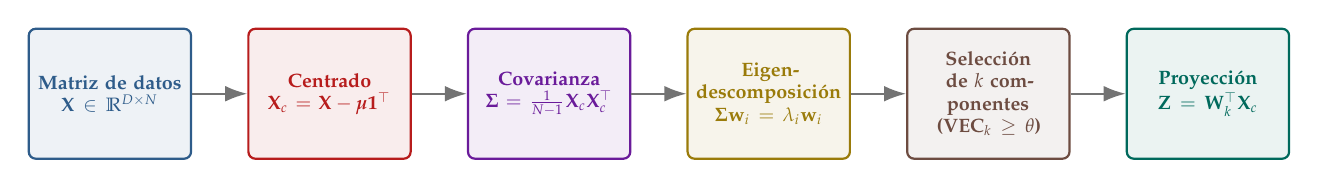
\begin{tikzpicture}[node distance=7mm]
				\node[box2=cBlue] (n1) {Matriz de datos\\$\mathbf{X} \in \mathbb{R}^{D\times N}$};
				\node[box2=cRed, right=of n1] (n2) {Centrado\\$\mathbf{X}_c = \mathbf{X}-\boldsymbol{\mu}\mathbf{1}^\top$};
				\node[box2=cPurple, right=of n2] (n3) {Covarianza\\$\boldsymbol{\Sigma} = \frac{1}{N-1}\mathbf{X}_c\mathbf{X}_c^\top$};
				\node[box2=cYellow, right=of n3] (n4) {Eigen-\\descomposición\\$\boldsymbol{\Sigma}\mathbf{w}_i = \lambda_i\mathbf{w}_i$};
				\node[box2=cBrown, right=of n4] (n5) {Selección\\de $k$ componentes\\($\text{VEC}_k \ge \theta$)};
				\node[box2=cTeal, right=of n5] (n6) {Proyección\\$\mathbf{Z} = \mathbf{W}_k^\top \mathbf{X}_c$};
				\foreach \a/\b in {n1/n2,n2/n3,n3/n4,n4/n5,n5/n6} \draw[arr] (\a) -- (\b);
		\end{tikzpicture}}
		\caption{Diagrama de bloques del algoritmo de PCA.}
		\label{fig:algoritmo}
	\end{figure}
	
	\begin{enumerate}[itemsep=4pt]
		\item \textbf{Estandarización / Centrado:} Calcular la media muestral $\boldsymbol{\mu}$ y centrar los datos mediante $\mathbf{X}_c = \mathbf{X} - \boldsymbol{\mu}\mathbf{1}^\top$. En casos donde las variables tengan unidades o escalas dispares, se normaliza cada fila para que presente desviación estándar unitaria.
		\item \textbf{Cálculo de la matriz de covarianza:} Obtener $\boldsymbol{\Sigma} = \frac{1}{N-1}\mathbf{X}_c\mathbf{X}_c^\top \in \mathbb{R}^{D \times D}$.
		\item \textbf{Descomposición espectral:} Determinar los pares propios $(\lambda_i, \mathbf{w}_i)$ para $i=1,\dots,D$ tales que $\boldsymbol{\Sigma}\mathbf{w}_i = \lambda_i\mathbf{w}_i$, ordenándolos de forma que $\lambda_1 \ge \lambda_2 \ge \dots \ge \lambda_D$. Alternativamente, calcular la descomposición en valores singulares (SVD) de $\mathbf{X}_c^\top / \sqrt{N-1}$.
		\item \textbf{Selección de la dimensión latente $k$:} Determinar $k$ mediante criterios heurísticos como el umbral de varianza explicada acumulada ($\text{VEC}_k \ge \theta$, comúnmente $\theta = 0.90$ o $0.95$) o el punto de inflexión en el gráfico de sedimentación (\emph{scree plot}).
		\item \textbf{Construcción de la matriz de transformación y proyección:} Formar $\mathbf{W}_k = [\mathbf{w}_1, \dots, \mathbf{w}_k] \in \mathbb{R}^{D \times k}$ y evaluar las coordenadas reducidas $\mathbf{Z} = \mathbf{W}_k^\top \mathbf{X}_c \in \mathbb{R}^{k \times N}$.
	\end{enumerate}
	
	\newpage
	
	% =================================================================
	% VENTAJAS Y LIMITACIONES
	% =================================================================
	\section{Propiedades, ventajas y limitaciones}
	
	\begin{table}[h!]
		\centering
		\caption{Comparativa de propiedades intrínsecas de PCA.}
		\label{tab:ventajas}
		\begin{tabular}{@{}p{6.6cm}p{6.6cm}@{}}
			\toprule
			\rowcolor{accent!85}
			\textcolor{white}{\textbf{Ventajas}} & \textcolor{white}{\textbf{Limitaciones}} \\
			\midrule
			Método completamente no supervisado: no requiere etiquetas de clase ni intervención heurística sobre los datos. & Transformación estrictamente lineal: no modela relaciones ni variedades no lineales intrínsecas en los datos. \\
			\addlinespace
			Garantiza la decorrelación ortogonal exacta de las variables proyectadas en el subespacio latente. & Criterio basado únicamente en varianza: las direcciones de máxima varianza no corresponden necesariamente con la máxima separabilidad de clases. \\
			\addlinespace
			Minimiza de manera óptima el error cuadrático medio de reconstrucción lineal (propiedad de Eckart-Young-Mirsky). & Sensible a la escala de medida: variables con magnitudes numéricas superiores dominan artificialmente los autovectores si no se estandariza. \\
			\addlinespace
			Proporciona una solución analítica exacta mediante descomposición espectral o SVD sin mínimos locales. & Pérdida de interpretabilidad física directa: las componentes son combinaciones lineales de todas las variables originales. \\
			\bottomrule
		\end{tabular}
	\end{table}
	\newpage
	\section{Conclusiones}
	
	El Análisis de Componentes Principales se consolida como una de las herramientas fundamentales del álgebra lineal aplicada al análisis multivariado y al aprendizaje automático. Su capacidad para desacoplar correlaciones lineales y ordenar la dispersión de los datos a lo largo de ejes ortogonales permite transformar representaciones redundantes en subespacios de dimensión reducida, preservando la máxima energía o varianza posible bajo transformaciones afines.
	
	Comprender su formulación lagrangiana, su estrecha equivalencia con la descomposición en valores singulares y sus supuestos de linealidad y escala resulta esencial tanto para su aplicación directa en compresión y visualización, como para el estudio de extensiones avanzadas (Kernel PCA, Probabilistic PCA y Sparse PCA).
	
	% =================================================================
	% BIBLIOGRAFÍA
	% =================================================================
	\newpage
	\renewcommand{\refname}{Bibliografía}
	\begin{thebibliography}{99}
		\addcontentsline{toc}{section}{Bibliografía}
		
		\bibitem{pearson1901} Pearson, K. (1901). On lines and planes of closest fit to systems of points in space. \textit{Philosophical Magazine}, 2(11), 559--572.
		
		\bibitem{hotelling1933} Hotelling, H. (1933). Analysis of a complex of statistical variables into principal components. \textit{Journal of Educational Psychology}, 24(6), 417--441.
		
		\bibitem{jolliffe2002} Jolliffe, I. T. (2002). \textit{Principal Component Analysis} (2nd ed.). Springer.
		
		\bibitem{bishop2006} Bishop, C. M. (2006). \textit{Pattern Recognition and Machine Learning}. Springer.
		
		\bibitem{duda2001} Duda, R. O., Hart, P. E., \& Stork, D. G. (2001). \textit{Pattern Classification} (2nd ed.). Wiley.
		
		\bibitem{strang2016} Strang, G. (2016). \textit{Introduction to Linear Algebra} (5th ed.). Wellesley-Cambridge Press.
		
	\end{thebibliography}
	
\end{document}